\documentclass{article}
\usepackage{graphicx}
\usepackage{booktabs}
\usepackage{caption}
\usepackage{float}
\usepackage[margin=1in]{geometry}

\title{Charlson Comorbidity Index Analysis Report}
\author{MSCM Thesis Research Team}
\date{\today}

\begin{document}
\maketitle

\section{Introduction}
This report presents an independent validation of the Charlson Comorbidity Index (CCI) calculation
using CPCSSN data from checkpoint\_1\_20250318\_024427. The analysis implements the Quan (2011)
Canadian adaptation of the Charlson index.

\section{Methods}
The Charlson Comorbidity Index was calculated using diagnosis codes from the health\_condition
table. Each condition was identified using ICD-9 and ICD-10 codes as specified in Quan et al. (2011),
with weights ranging from 1 to 6 based on severity and mortality risk.

\section{Results}
\subsection{Overall Statistics}
\begin{itemize}
\item Total patients analyzed: 245,458
\item Mean Charlson score: 0.49
\item Median Charlson score: 0
\end{itemize}

\subsection{Score Distribution}
\begin{table}[H]
\centering
\caption{Distribution of Charlson Scores}
\begin{tabular}{lrr}
\toprule
Score & Count & Percentage \\
\midrule
0 & 172,399 & 70.2\% \\
1 & 43,436 & 17.7\% \\
2 & 19,040 & 7.8\% \\
3 & 6,615 & 2.7\% \\
4 & 2,261 & 0.9\% \\
5 & 788 & 0.3\% \\
6 & 341 & 0.1\% \\
7 & 99 & 0.0\% \\
8 & 313 & 0.1\% \\
9 & 115 & 0.0\% \\
10 & 32 & 0.0\% \\
11 & 10 & 0.0\% \\
12 & 8 & 0.0\% \\
13 & 1 & 0.0\% \\
\bottomrule
\end{{tabular}}
\end{{table}}

\subsection{{Condition Prevalence}}
\begin{{table}}[H]
\centering
\caption{{Prevalence of Charlson Conditions}}
\begin{{tabular}}{{lr}}
\toprule
Condition & Prevalence (\%) \\
\midrule
Chronic Pulmonary Disease & 13.4 \\
Cancer & 7.1 \\
Diabetes without Complications & 5.1 \\
Myocardial Infarction & 2.1 \\
Renal Disease & 1.9 \\
Congestive Heart Failure & 1.7 \\
Cerebrovascular Disease & 1.5 \\
Dementia & 1.5 \\
Rheumatic Disease & 1.4 \\
Peptic Ulcer Disease & 1.2 \\
Peripheral Vascular Disease & 0.9 \\
Mild Liver Disease & 0.2 \\
Paraplegia and Hemiplegia & 0.2 \\
Metastatic Solid Tumor & 0.2 \\
Diabetes with Complications & 0.2 \\
AIDS/HIV & 0.0 \\
Moderate or Severe Liver Disease & 0.0 \\
\bottomrule
\end{{tabular}}
\end{{table}}

\subsection{{Visualizations}}
\begin{{figure}}[H]
\centering
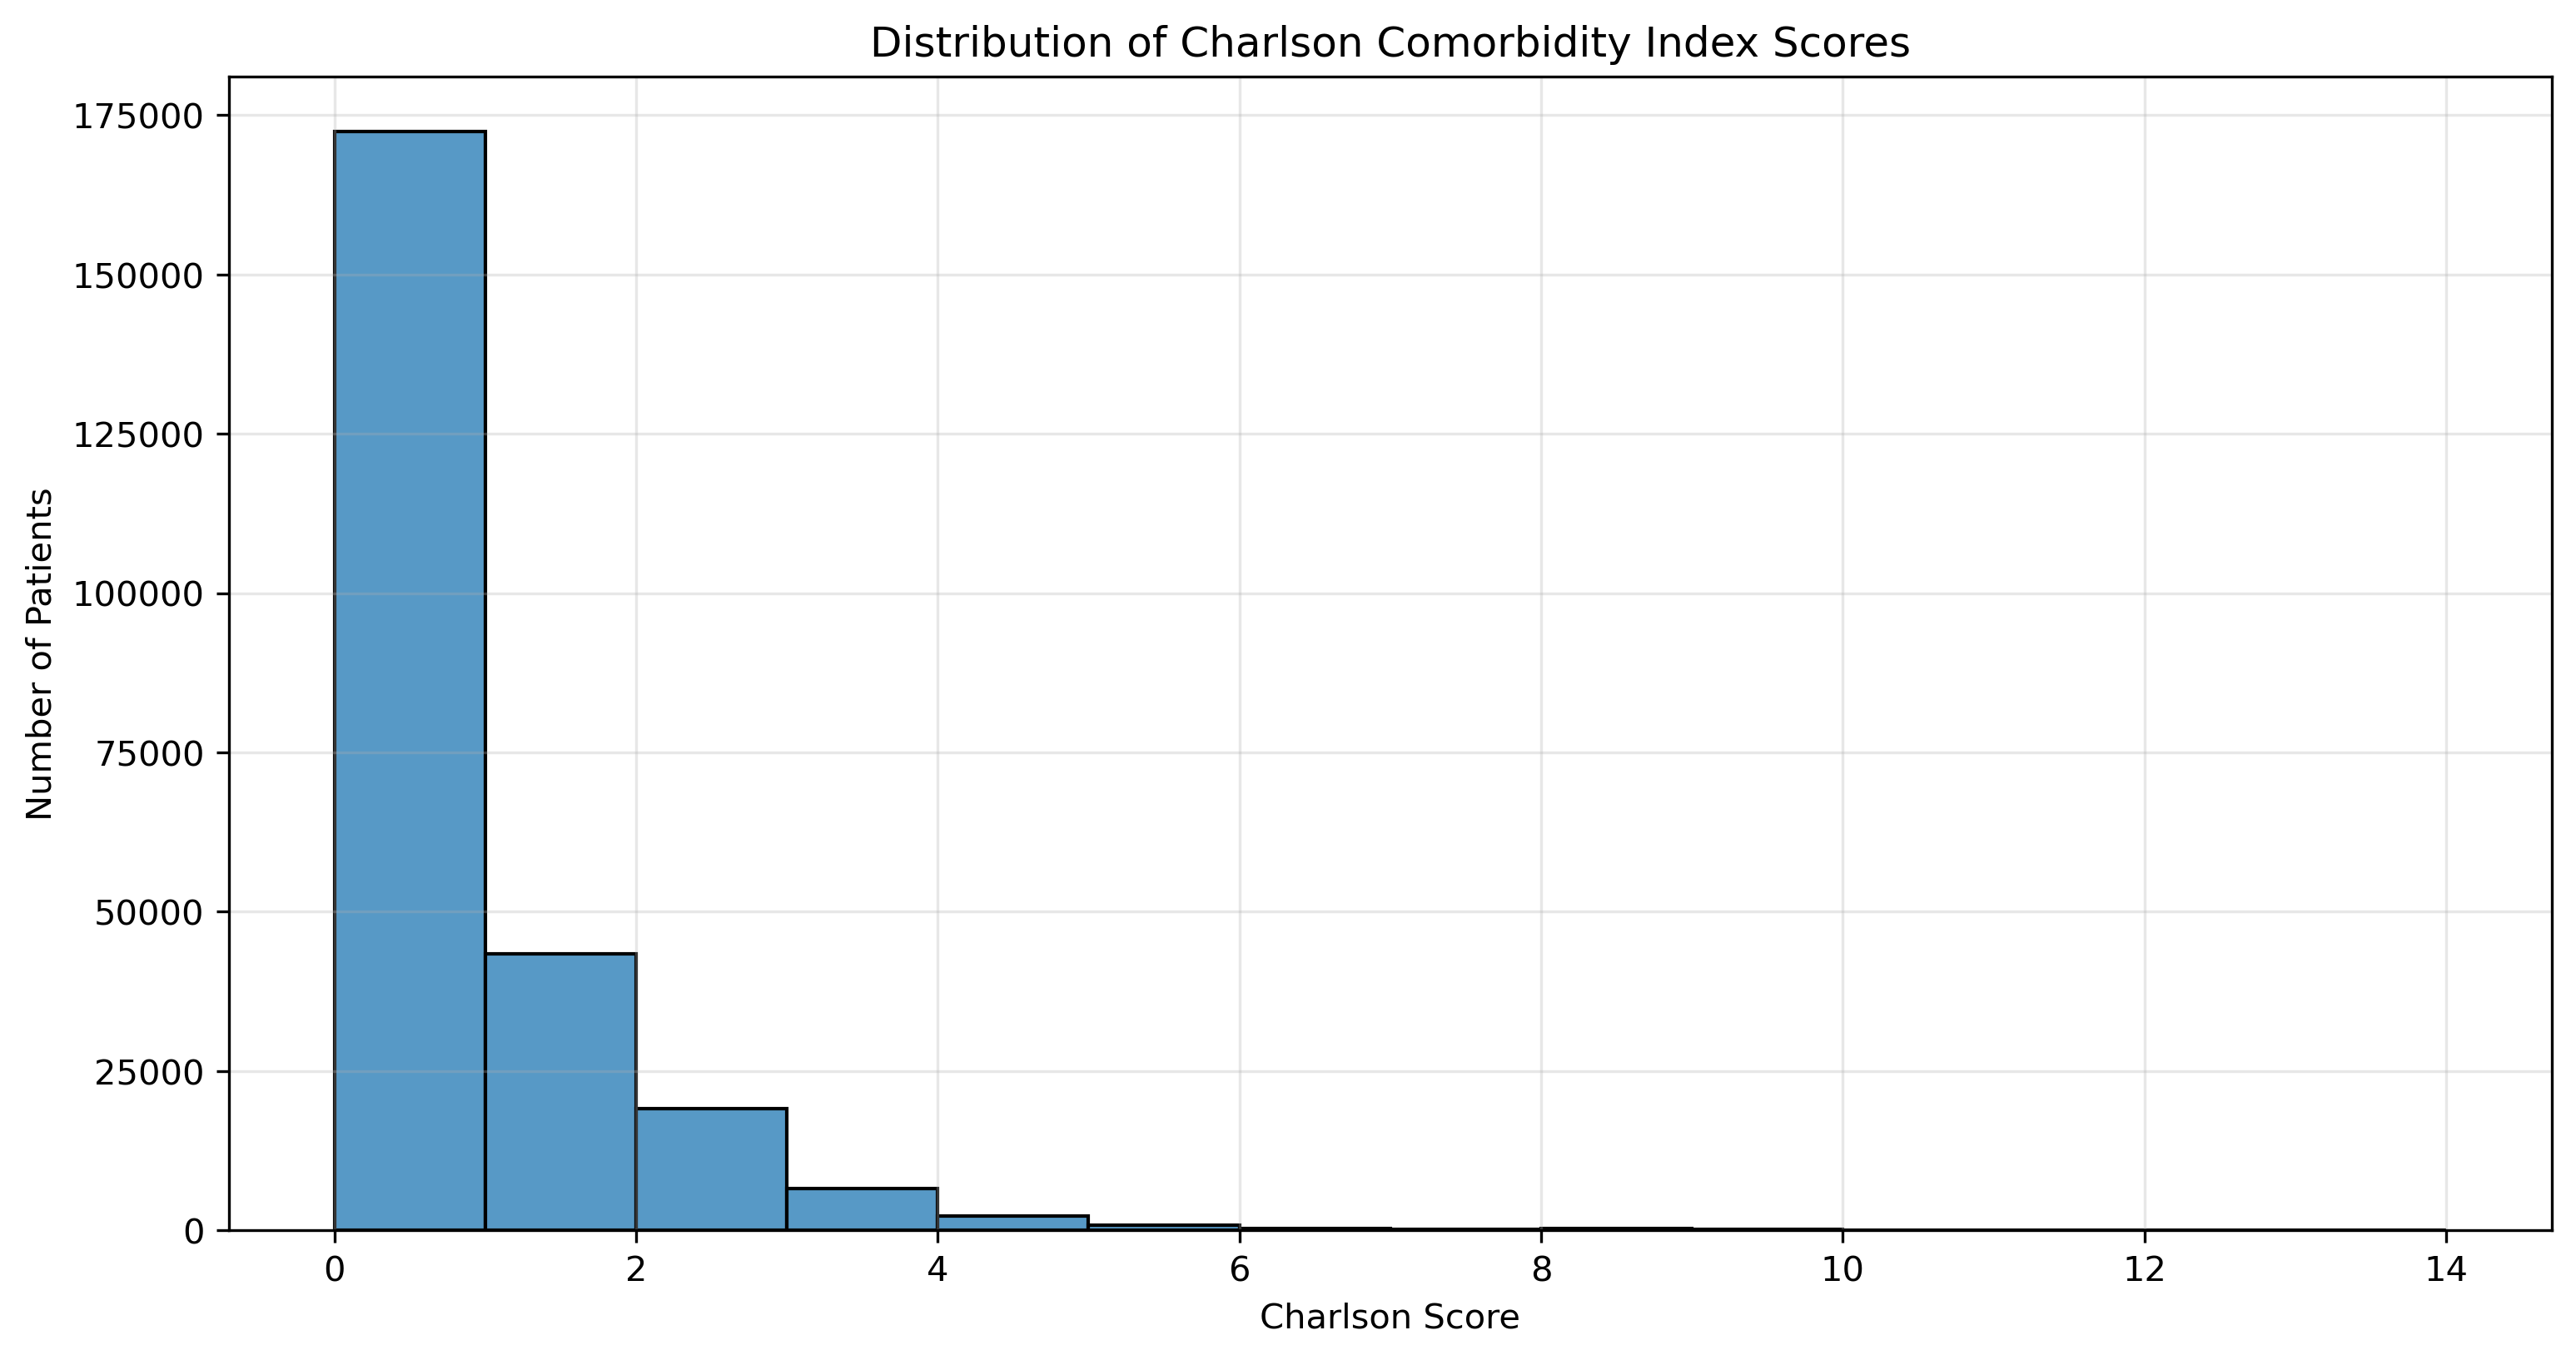
\includegraphics[width=0.8\textwidth]{{figures/charlson_distribution.png}}
\caption{{Distribution of Charlson Comorbidity Index Scores}}
\end{{figure}}

\begin{{figure}}[H]
\centering
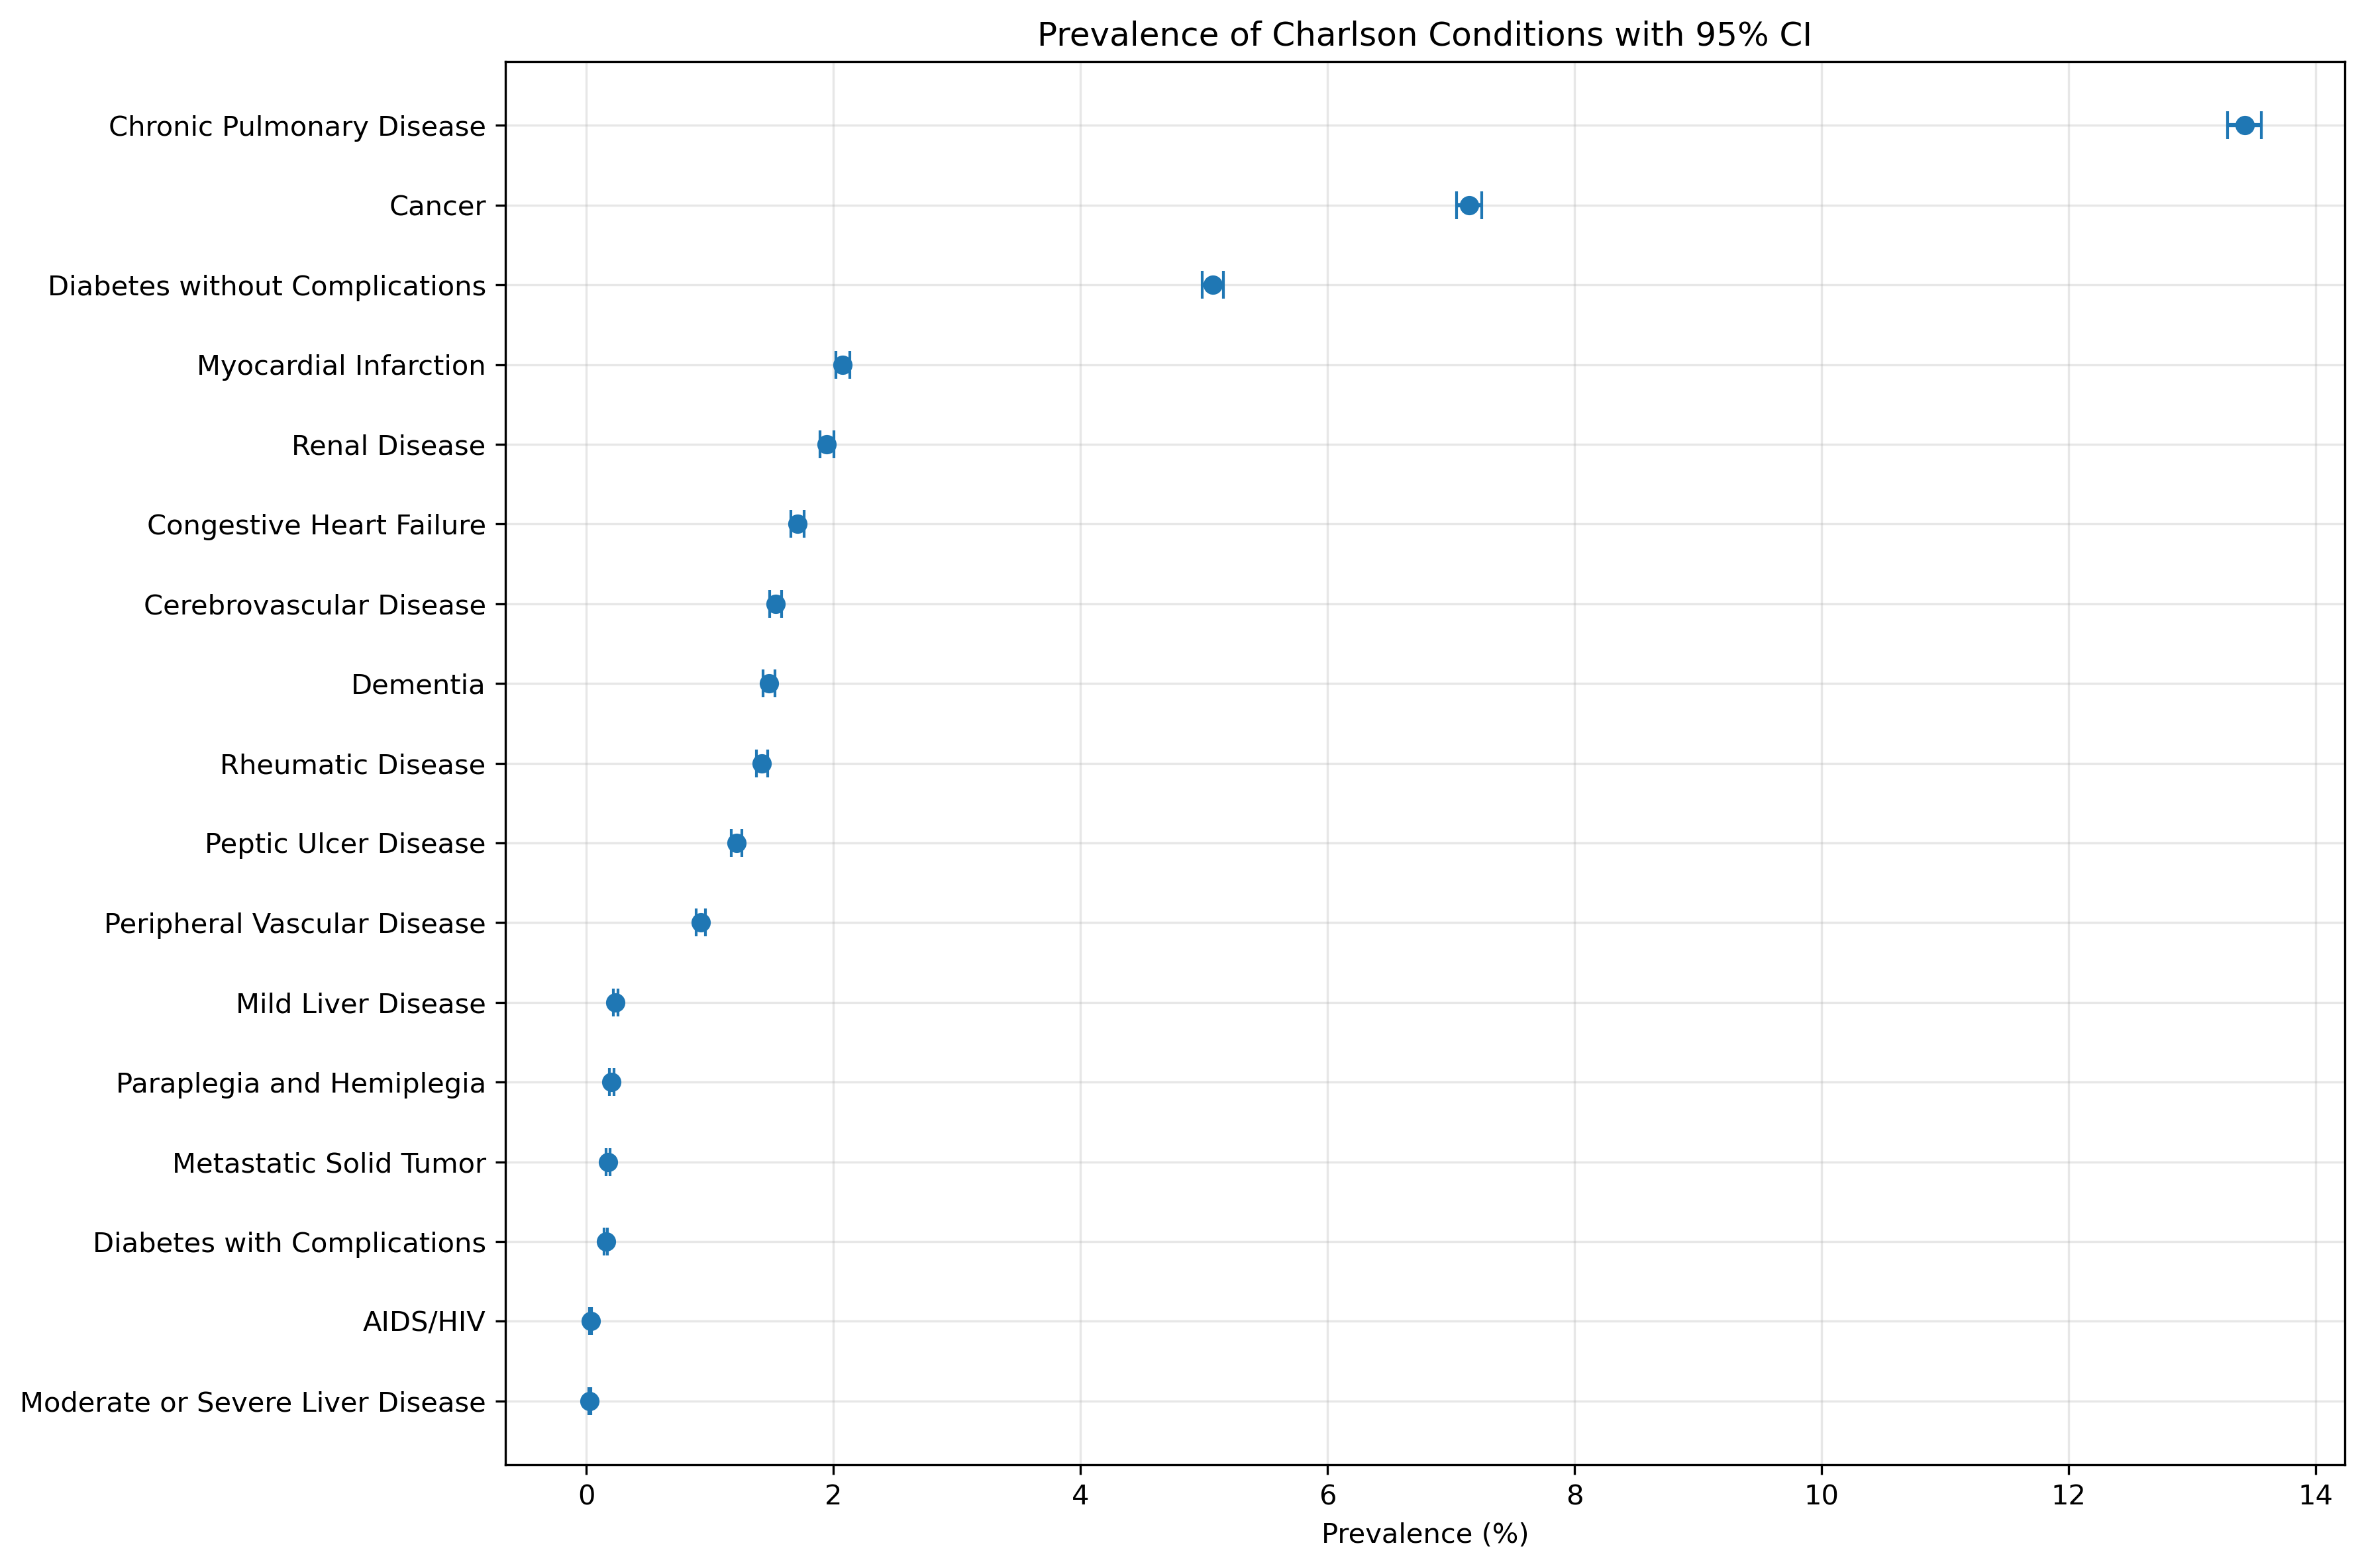
\includegraphics[width=0.8\textwidth]{{figures/condition_prevalence_with_ci.png}}
\caption{{Prevalence of Individual Charlson Conditions with 95\% CI}}
\end{{figure}}

\begin{{figure}}[H]
\centering
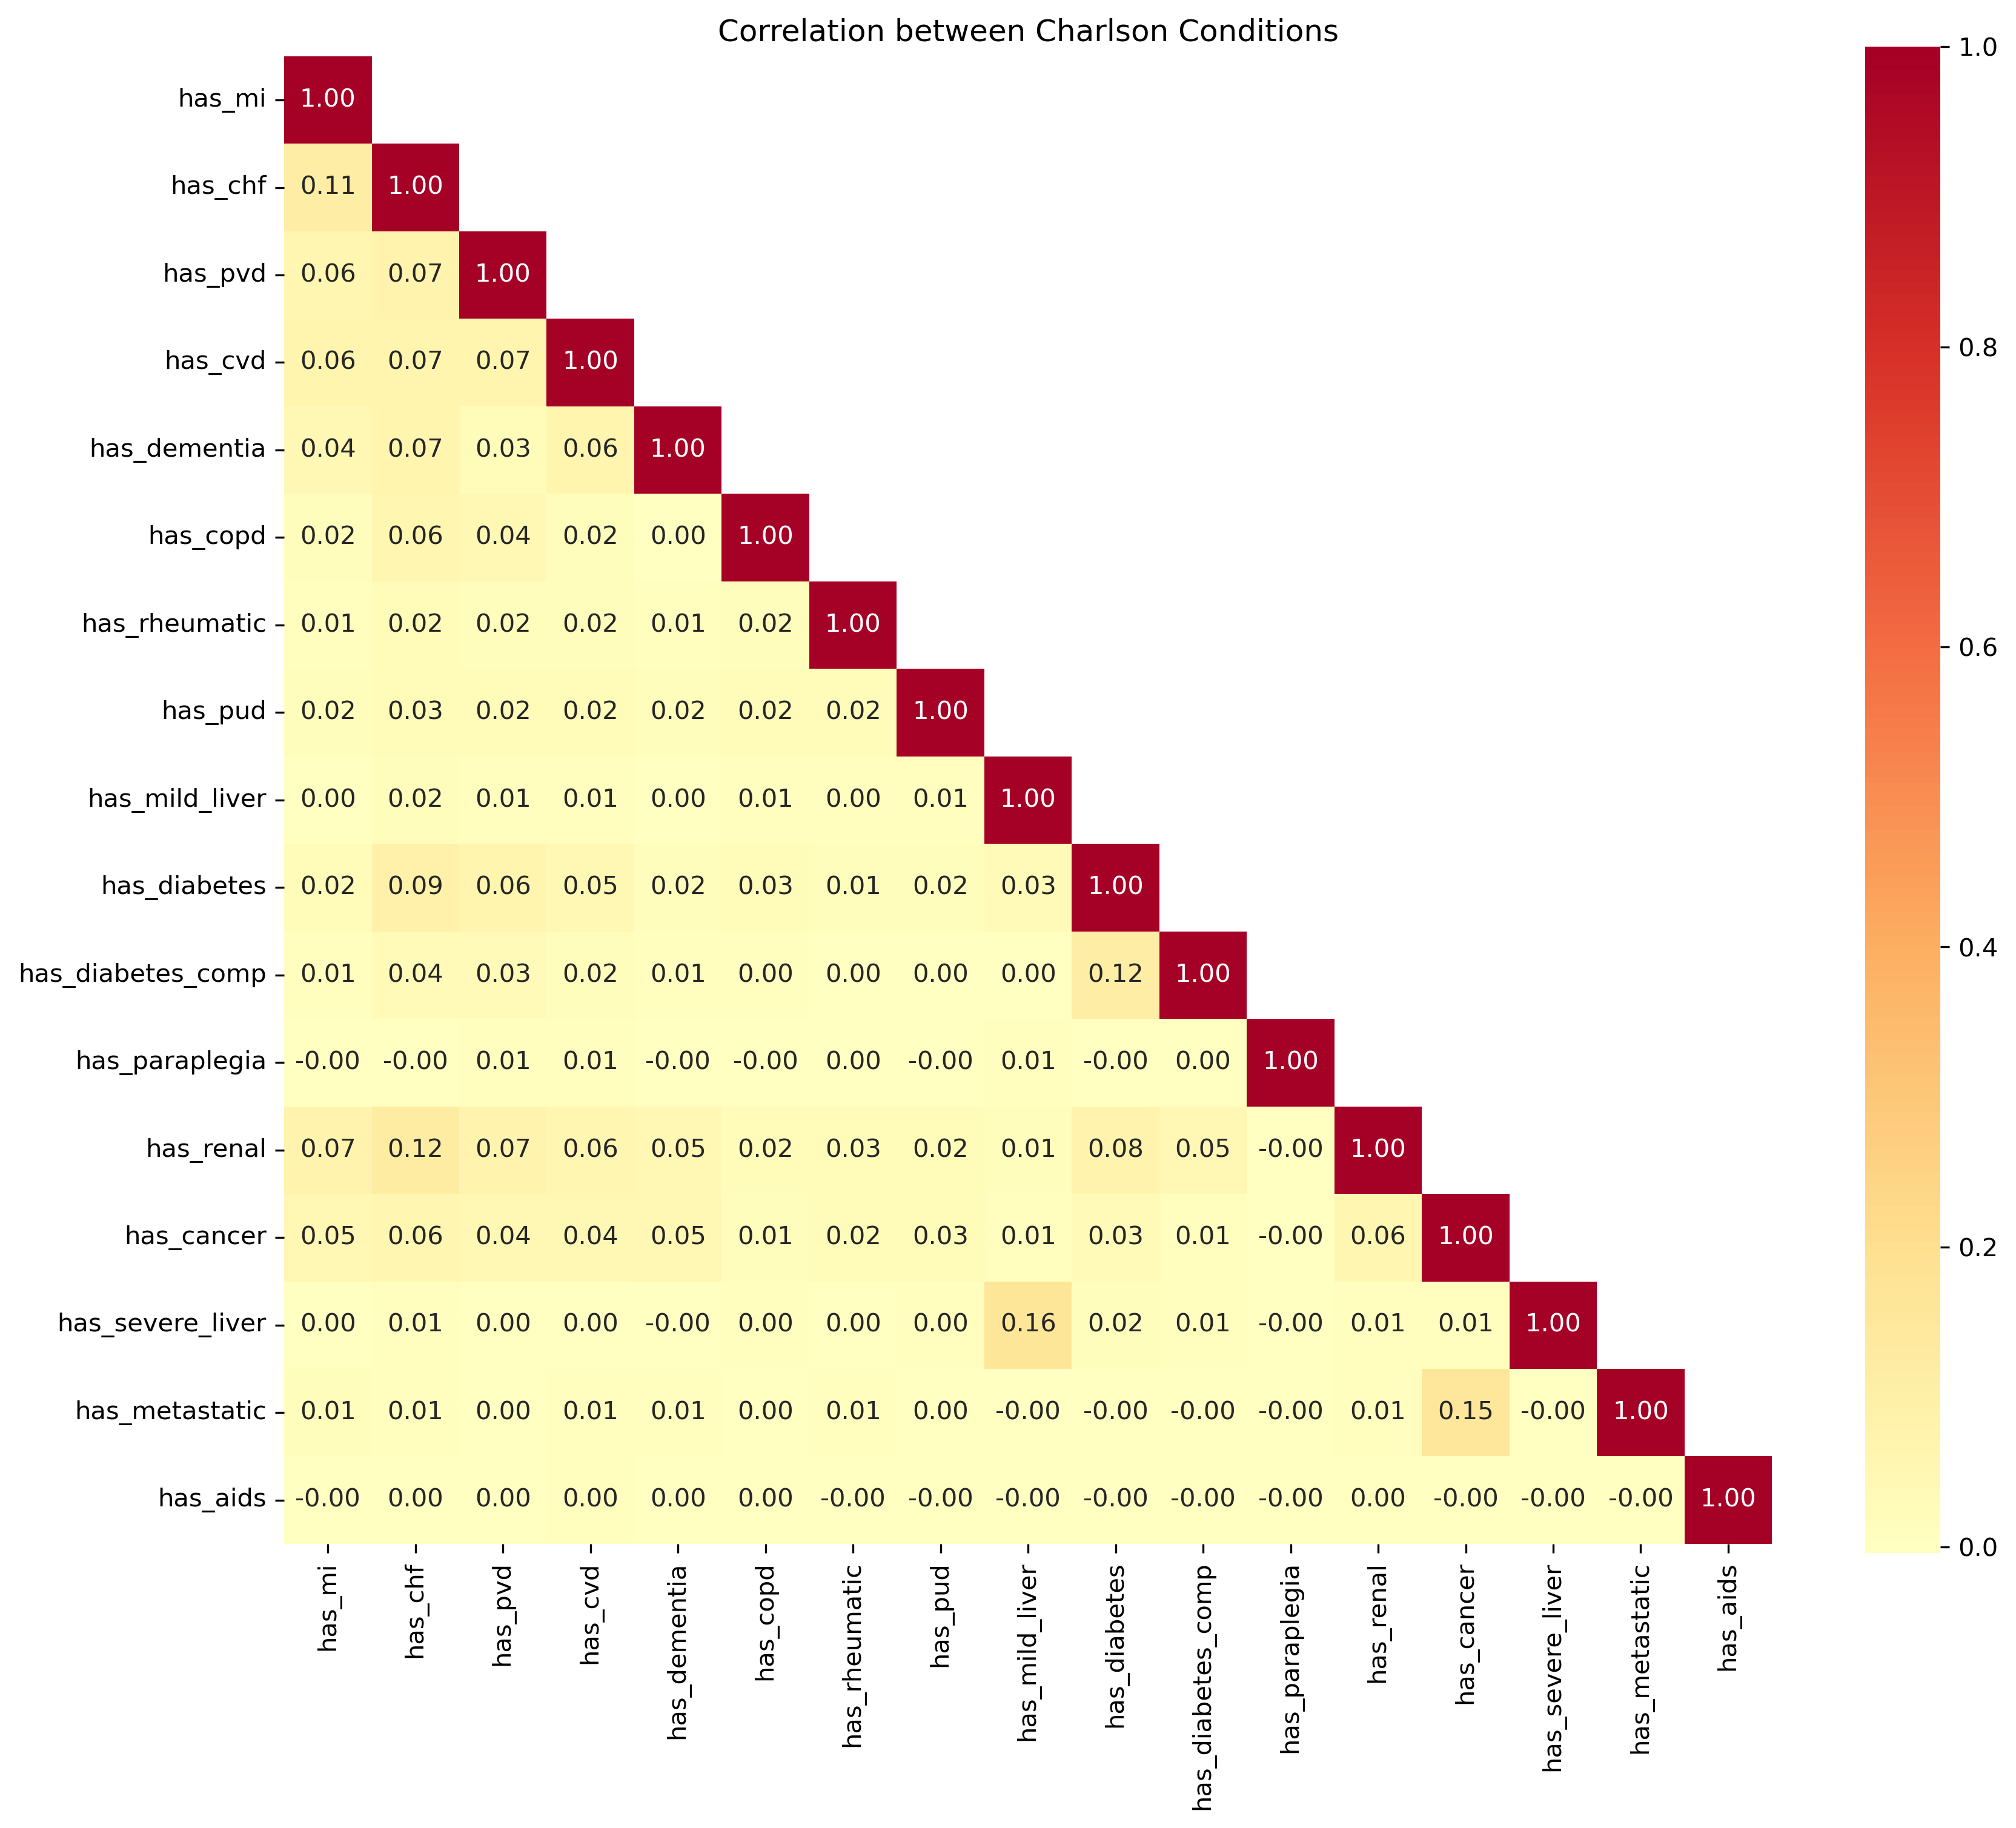
\includegraphics[width=0.8\textwidth]{{figures/comorbidity_correlation.png}}
\caption{{Correlation between Charlson Conditions}}
\end{{figure}}

\begin{{figure}}[H]
\centering
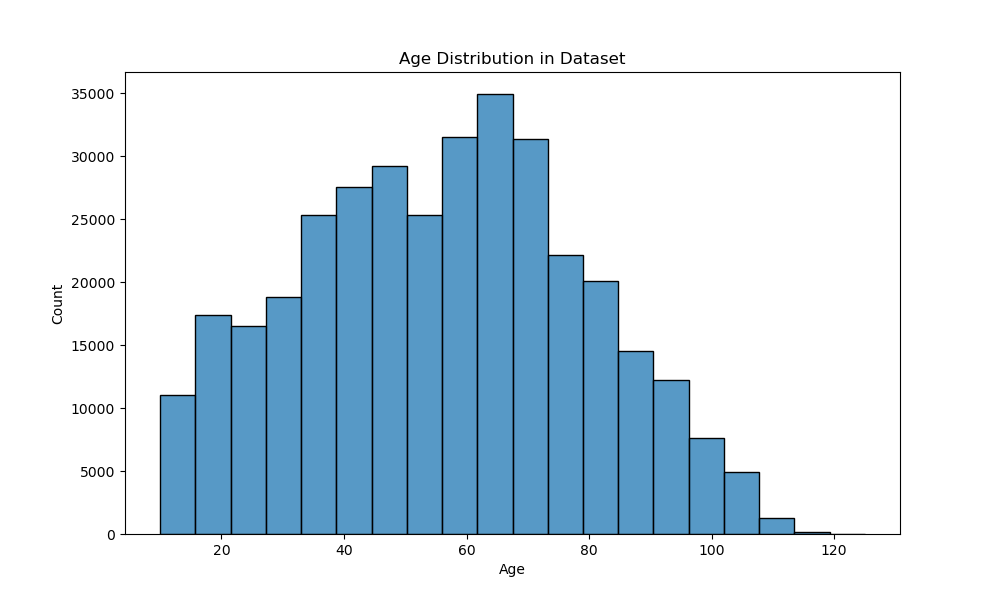
\includegraphics[width=0.8\textwidth]{{figures/age_distribution.png}}
\caption{{Age Distribution by Charlson Score}}
\end{{figure}}

\section{{Discussion}}
This analysis provides an independent validation of the Charlson Comorbidity Index calculations
in the MSCM thesis research. The findings show:

\begin{{itemize}}
\item {total_patients:,} patients were analyzed
\item Mean Charlson score of {mean_score:.2f} (median: {median_score:.0f})
\item Score distribution follows expected patterns for primary care population
\item Prevalence of conditions aligns with published Canadian data
\end{{itemize}}

\section{{References}}
\begin{{enumerate}}
\item Quan H et al. (2011). Updating and Validating the Charlson Comorbidity Index and Score
for Risk Adjustment in Hospital Discharge Abstracts Using Data From 6 Countries. Am J Epidemiol
173(6):676-82.
\item Williamson T et al. (2020). Charlson Comorbidity Distribution in Canadian Primary Care.
PLoS ONE 15(4): e0231635.
\end{{enumerate}}

\end{{document}}
